\documentclass{article}
\usepackage[utf8]{inputenc}
\usepackage[polish]{babel}
\usepackage{polski}
\usepackage{float}
\usepackage{enumerate}
\usepackage{enumitem}
\usepackage{natbib}
\usepackage{graphicx}
\usepackage{geometry}
\usepackage{pdfpages}
\newgeometry{tmargin=2.5cm, bmargin=2.5cm, lmargin=2.5cm, rmargin=2.5cm}

\title{Kompas elektroniczny}
\author{Dawid Brząkała}
\date{}

\begin{document}
\maketitle

\section{Cel projektu}
Celem projektu jest stworzenie wizualizacji kompasu w 3D oraz wizualizacji danych pomiarowych w postaci wykresu. Dane będą dostarczane do programu z zewnętrznego układu z mikroprocesorem oraz akcelerometrem i magnetometrem co pozwoli na uzyskanie danych o przechyleniu urządzenia oraz kierunku południka magnetycznego.

\section{Założenia projektu}
Układ pomiarowy zostanie zaprogramowany na płytce rozwojowej STM32F3 Discovery wyposażonej w peryferia wymagane do projektu. Odczyt pomiarów, jak i konfiguracja akcelerometru oraz magnetometru realizowana jest poprzez magistralę $I^2C$. Komunikacja układu z komputerem odbędzie się poprzez kabel USB i protokół RS-232. Dane wysyłane będą bitowo, przeznaczając 4 bajty na każdy pomiar i sumę kontrolną typu float. Ramka z danymi rozpoczęta zostanie przez znak 'X' oraz zakończona sumą kontrolną, będącą sumą  wartości przesyłanych pomiarów.
\section{Funkcjonalności aplikacji}

\section{Harmonogram}
\begin{figure}[H]
  \centering
  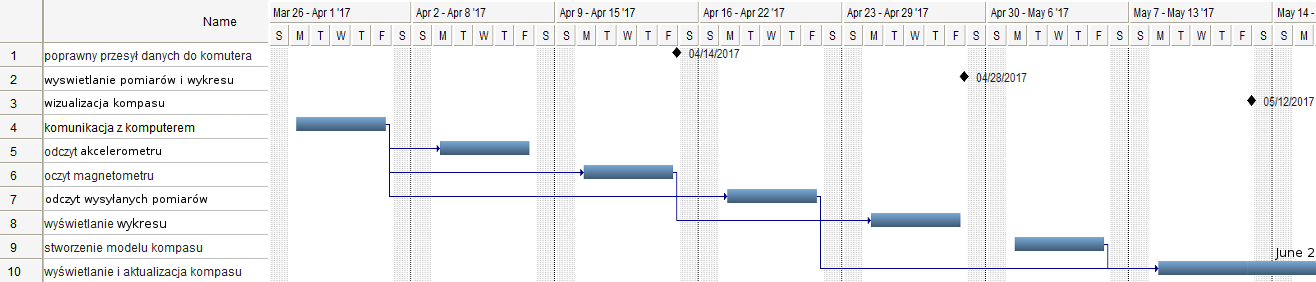
\includegraphics[width=\linewidth]{wds.png}
\end{figure}

\section{Kamienie milowe}
\begin{itemize}[noitemsep]
\item Poprawny przesył danych do komputera
\item Wyświetlanie pomiarów oraz wykresu
\item Wizualizacja kompasu
\end{itemize}

\section{Zrealizowane zadania}
\begin{itemize}[noitemsep]
\item Komunikacja z komputerem
\item Odczyt akcelerometru
\item Odczyt magnetometru
\item Odczyt wysłanych pomiarów
\item Wyświetlanie wykresu
\item stworzenie modelu kompasu
\end{itemize}

\section{Szkic interfejsu graficznego programu}
\begin{figure}[H]
  \centering
  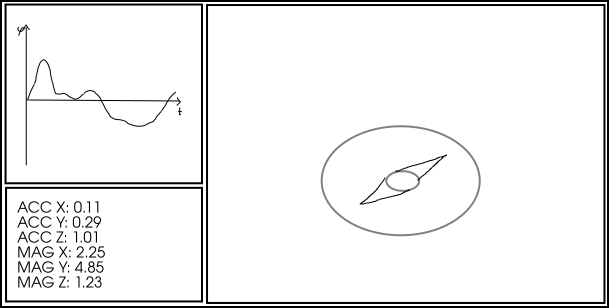
\includegraphics[width=0.75\linewidth]{layout.png}
\end{figure}

\begin{figure}[H]
\section{Diagram UML}
  \centering
  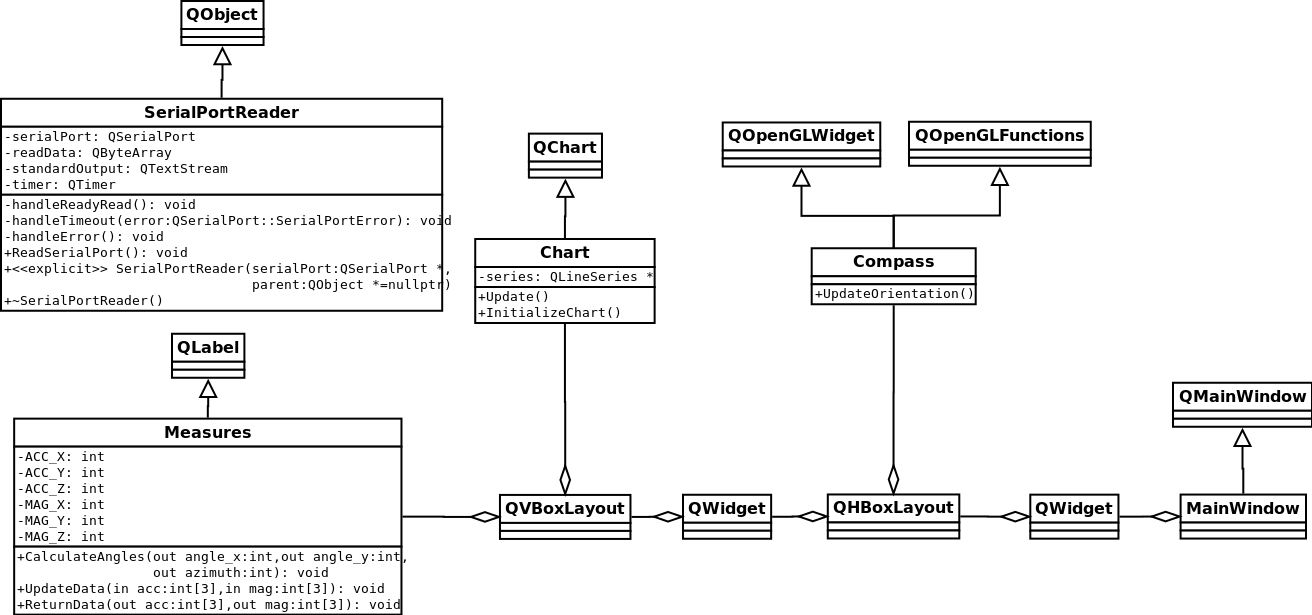
\includegraphics[width=0.75\linewidth]{Diagram1.png}
\end{figure}

\begin{figure}[H]
\section{Schemat blokowy}
  \centering
  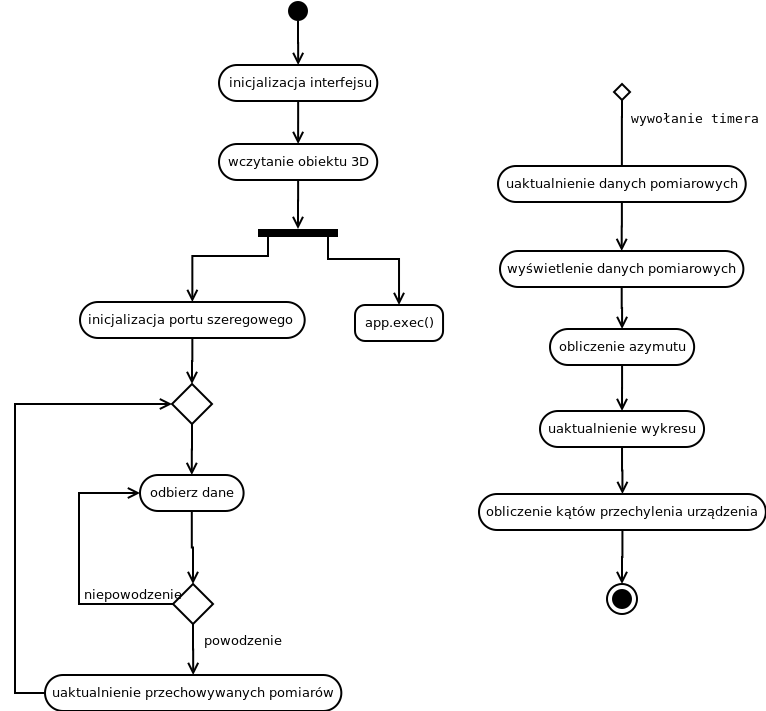
\includegraphics[width=0.75\linewidth]{Diagram2.png}
\end{figure}

